\documentclass[10pt,conference]{IEEEtran}

\usepackage{hyperref}
\usepackage{graphicx}	% For figure environment
\usepackage[T1]{fontenc}

\begin{document}
\title{Sentiment Analysis of Tweets}

\author{
  Dino Mujkic, Hrvoje Busic, Sebastijan Stevanovic\\
  \textit{Department of Computer Science, EPFL, Switzerland}
}

\maketitle

\begin{abstract}
Our research project focused on sentiment analysis of a large corpus of tweets (messages and announcements) from the popular social media site Twitter. The task was to predict whether the sentiment of a tweet was positive or negative, more specifically, whether the user had used a positive or negative smiley face. With this endeavor as the main objective, this report will represent our comprehensive study of the different methods to preprocess the text within tweets, represent words as appropriate features, and produce an optimal algorithm through evaluation of several machine learning classification techniques. Numerous tests and combinations of the above processes allowed us to obtain a much deeper understanding of our datasets, natural language processing and ultimately resulted in an algorithm which achieved a high classification accuracy on the test dataset.
\end{abstract}

\section{Introduction}

Natural Language Processing (NLP), an increasingly expanding and developing field of artificial intelligence, has been gaining increasing popularity and value in the modern world. Speech recognition, natural language understanding and generation, are tasks that are no longer just a focus within of academic communities, but an important part of the modern commercial sector, in particular for companies such as Google, Facebook and Amazon which are at the forefront of innovating how humans interact with computers and with others through technology.
An important area of NLP is sentiment analysis, more specifically, understanding the human emotions behind written and spoken words. While it is known that certain words are integral to how we express different sentiments, the task is immensely difficult to generalize due to the complexities of natural language as well as the wide spectrum of human emotions. Nonetheless, important strides have been made in recent years, largely thanks to an augmented ability of computers to process and understand sentence semantics and different contexts for individual words as well as within interactions between several words.
Our task focuses on understanding the sentiment of a tweet, a relatively more difficult task than simple written text due to the informal nature of tweets and use of emoticons as well as hashtags (tags that start with " \# " and are composed of one or multiple words). Through this report, we aim to present the different approaches to preprocessing, evaluation and classifying of tweets, and understand their pros and cons in an effort to yield optimal results.


\section{Datasets and Data Description}
\label{sec:data-structure}

The training dataset consists of 2.5 million tweets separated into two files, with equal division of positively and negatively classified tweets. More specifically, each file consists of 1.25 million tweets that contained smiley faces which were either positive ":)", or negative ":(", and had reflected the original sentiment of the tweet. The dataset used for testing consists of 10 000 unlabeled tweets which need to be categorized according to their original sentiment. Using the already categorized training tweets, we are asked to use the text contained within them to produce and train a classifier that is able to infer sentiment for the test dataset and hence for future tweets as well.
 
The fact that tweets with positive and negative sentiment are equally distributed in the training dataset, as well as the absence of neutral sentiment, made our training and evaluation tasks for different classifiers easier and more successful. However, it should be noted that results produced through our research project focus specifically on the type of tweets which included the positive or negative smileys, not necessarily tweets in general.
 
Furthermore, tweets themselves have unique properties which need to be taken into account during analysis. Twitter posts are social media announcements written by everyday people. The language of the tweets is overwhelmingly informal, often containing abbreviations, collocations and other word conjugations and representations which are not used in the standard English language. Symbols, emoticons and other special characters add to the meaning and are usually the crux of the message that the author is trying to relay to other users. Hashtags (\#) followed by text are used to mark topics and themes with which an author relates his or her message. Furthermore, grammatically incorrect sentences, mispronounced words and other common mistakes, point to the importance of preprocessing steps in order to get closer to a more normalized and useful dataset.

\section{Text Preprocessing Methods}
\label{sec:preprocessing}

In this section we provide an outline of implemented methods aimed at preprocessing tweets in order to obtain content which, after vectorization, would score better with explored classification models by more clearly conveying the author's original sentiment.

It is important to emphasize that these methods were not designed to be used at the same time, but to provide us with a unique toolbox with which we can explore different combinations of tweet preprocessing techniques and classifiers. Methods which utilize so called 'tags' (content between '<' and '>' symbols) were heavily inspired by Stanford's pretrained \textit{GloVe} word embeddings which we will discuss in depth later on.
 
\textbf{Filtering existing '<user>' and '<url>' tags:} We have implemented methods which remove existing '<user>' and '<url>' tags respectively in order to investigate how do those tags, which came prepared with the data set, impact quality of the sentiment classification.

\textbf{Emoticon analysis:} Emojis are widely used in social media posts, and natively convey the author's sentiment. We have implemented two approaches to extracting the sentiment present in these symbols. First approach places a descriptive tag in front of emoticon (e.g. '<smile>'), while the second approach replaces emoticon with sentiment words, words 'positive' and 'negative' as it is appropriate in case of emoji, in order to clearly convey more general sentiment connected to the emoji.

\textbf{Stop-word and small-words filtering:} Stop words are common words in the English language that are present in every tweet and thus do not imply any sentiment, for which reason they can be removed during analysis. Moreover, small-words (words only 1 character long) can also be removed.

\textbf{Tagging hashtags and numbers:} Hashtags and numbers can be marked with preceeding tag,  '<hashtag>' and '<number>' respectively, in order to mark their position in the tweet, and indicate their earlier existence in case of further processing.

\textbf{Splitting hashtags:} Hashtags are concatenated words used to mark topics and themes with which an author relates his or her message. For this reason we implemented method which tries to split the content of the hashtag by using the dictionary with most frequently used English words in descending order, according to Zipf's law.

\textbf{Removing numbers:} Words in tweet which contain number in them can be exchanged for the tag '<number>'. 

\textbf{Emphasizing sentiment words:} Assisted by two lexicons, containing words with clearly positive and clearly negative sentiments respectively, we have implemented a method that searches for words within tweets that appear in those lexicons in order to emphasize them, while more clearly pointing to the sentiment of the author.

\textbf{Emphasizing repeated characters and punctuation:} Successive repetition of letters within a word as well as punctuation symbols points to author's sentiment. For this reason we have implemented a method which emphasizes those occurrences by placing an appropriate tag alongside them. Moreover, additional method allows for replacing a word that experiences letter repetitions with two occurrences of the standard form of that word, in that way hoping to emphasize sentiment that that word carries.

\textbf{Lemmatization and stemming:} Methods which apply lemmatization and stemming separately have been implemented in order to homogenize words being in different tenses and forms.


\section{Feature Extraction and Tweet Representation}
\label{sec:tweet-representation}

As briefly mentioned before, to use the different machine learning models, it is necessary to convert our tweets in text representation to numerical features, namely vectors that are numerical representations of words and in turn, tweets. In more formal terms, we want to represent our datasets into matrices of the form $N \times D$, where \textit{N} is the number of data points (tweets) and \textit{D} is the dimension of our vector representation. Below, we present several explored algorithms to achieve our vector numerical representation.

\subsection{TF-IDF}
In an effort to obtain semantic and contextual information for individual words, we are able to utilize the "Term Frequency - Inverse Document Frequency \textit{(TF-IDF)}" representation. \textit{TF-IDF} gathers this information by calculating the frequency of a word compared to its inverse proportion within the entire text corpus. The benefit of this representation is that it can be combined with others by decreasing or increasing the significance of certain words based on its \textit{TF-IDF} value where more representative words are distinguished from common ones.

\subsection{N-grams}
In an effort to further gather contextual information of a word we can combine continuous words into representative sequences as certain words often appear together in specific contexts. The manner in which we do this specifically is by combining a number n of words into a sequence (i.e., for $n=4$ we get \textit{4-grams}).

\subsection{Word Embeddings}
A relatively novel representations of text is in the form of word embeddings (\textit{WE}) which are essentially vector representation of words using real numbers. The idea behind these word embeddings is to recognize words that appear in similar context and thus, words of similar semantic and contextual significance will have vectors with highly similar values. As the size of these vectors is essentially arbitrary since they are just collections of generated real numbers, this method has the advantage of allowing us to select the depth of the contextual analysis for each word. For our research we decided opted for dimensionality $D=200$ since this is the highest standard number for dimensionality and which had a very useful pretrained vectors available from Stanford, namely \textit{GloVe}. However, we also decided to test producing our own word embeddings using another recently highly optimized and effective algorithm developed at Google, namely \textit{Word2vec}. We now discuss more in depth each of these vector embeddings and their usage.

\subsubsection{GloVe Pretrained}
\textit{GloVe} is an unsupervised learning algorithm for obtaining vector representations for vectors originating from Stanford. By using this algorithm on 2 billion tweets, vectors with dimensionality $D=200$ for 1.2 million words was obtained and is readily available for the public to use. During our data preparation process, we load the values of each of these vectors (word embeddings) to use them for representing our tweets in matrix format with numerical values which we will discuss afterwards more in depth.

\subsubsection{Word2vec}
\textit{Word2vec} is a group of related models that are used to produce word embeddings developed by a team of researchers at Google. This algorithm is highly optimized and thus suitable for testing as well as being very effective. It is readily available from the internet and during our data presentation, we trained it on the entire corpus of our data to obtain word embeddings for each word in our corpus vocabulary, again with the aim of obtaining a proper tweet representation.

\subsubsection{Word2vec and TF-IDF}
As we mentioned before, a benefit of the \textit{TF-IDF} algorithm is that it is possible to combine its values with other word representation. Hence, during our testing we attempted to improve the word embeddings obtained through \textit{Word2vec} by also multiplying them with their corresponding \textit{TF-IDF} values to achieve an even higher contextual significance for which word. Essentially, combining with \textit{TF-IDF} would change increase or decrease the significance of the values in a word embedding depending on the word's relevance or commonality.

\subsection{Tweet Representation}
The methods we described prior for obtaining vector and numerical representations of our text, or more specifically individual words, allow us to now represent entire tweets in a similar fashion. Essentially, since each tweet is a combination of words, a tweet representation would then be a combination of individual representations of those words (i.e. the words' embeddings). During our data preparation stages we attempted several different methods for combining the individual word representations, namely aggregation, averaging and vector expansion of the input. In the end, we found that best results are achieved by the last method, namely to simply input an expanded vector representation of a tweet to our neural network algorithms in the sense that each tweet was a matrix containing all of its words' embeddings.


\section{Classification Methods}

We have started our research with large set of different classifiers: Naive Bayes, Multinomial Naive Bayes, Support Vector Machines, Neural Networks and Convolutional Neural Networks.  Furthermore, start of our research included exploration of different classifiers and text representation combinations, with the latter being described earlier. After preliminary tests to get a hold of performance of different text vectorization methods, we have continued our exhaustive research with the word embeddings approach backed by Stanford's \textit{GloVe} word embeddings dictionary, with focus on \textit{Support Vector Machines}, \textit{Neural Networks} and \textit{Convolutional Neural Networks} classifiers.

\subsection{Support Vector Machines (SVM)}
SVM is a supervised machine learning algorithm that can be employed for both classification and regression purposes. SVMs are based on the idea of finding a hyperplane that best divides a dataset into two classes. Support vectors are the data points nearest to the hyperplane, the points of a data set that, if removed, would alter the position of the dividing hyperplane. They can be applied both as linear binary classifiers and nonlinear complements after kernel-trick. In our research we have relied on scikit's SVM implementation in Python, due to its high configurability, reliable documentation and support. For training we have configured classifier with the penalty parameter \textit{C} set at 1 and at most $1000$ iterations per run.

\subsection{Neural Networks (NN)}
NNs are a machine learning algorithm providing the ability of approximation of linear and nonlinear functions, with the use of backpropagation algorithm for learning. Network is built out of layers, with each layer consisting of neurons, while being highly configurable through selection of size and number of layers, as well as neurons within those layers. In our classification, we have relied on scikit's implementation of multilayered neural networks, for the same reasons as stated earlier. For training we have used \textit{SGD} algorithm, with learning rate set at $10^{-4}$, converging threshold set at $10^{-6}$, and at most $1000$ iterations per run.

\subsection{Convolutional Neural Networks (CNN)}
A relatively recent new player on the machine learning stage, CNNs have achieved great strides in improving the performance of deep-learning applications in certain areas, most notably in computer vision but NLP as well. In order to apply CNNs for our specific task, we needed to modify our textual representation of tweets by assume a maximum number of words in each tweet (this was achieved through padding). Additionally, through a numerical representation of each word in the sense of contextual relations between individual words, our final input representation becomes $m \times N$, where m is the max number of words and N is the dimension of individual word vectors (in our case, we opted to use $N=200$ and the pretrained \textit{GloVe} word embeddings). CNNs have several different types of layers which in combination should process and reduce the input size in a reasonable manner to apply a softmax classifier as the final step. During our testing stage, we tested several different layer configurations, batch sizes as well as the number of epochs which we present in the next section. It is important to note that our CNN testing and implementation was based on \textit{Tensorflow}, an open source library for data processing and computation.

\section{Observations and Results}

In this section, we will present the various results we obtained through exploration of different methods of text preprocessing, tweet representation and classification. The majority of our research focused on preprocessing as once we had setup a pipeline to evaluate different machine learning algorithms, the decisions and assumptions made during the preprocessing stage often had the most impact on the actual results, in comparison to parameter changes for the algorithms.

Firstly, we will present several text preprocessing techniques which had significantly improved or deteriorated the results of the trained classifiers. One assumption proved to be critically wrong and would severely hamper any algorithm with which it was attempted. This was the assumption that duplicate tweets from the training dataset do not yield additional information and hence should be removed. However, it was quickly shown that this was incorrect and that the duplicate tweets were essential to the strengthening of the training models. Additionally, it proved essential to distinguish between positive and negative words, adding appropriate emphasis with an adjacent sentiment word, 'positive' or 'negative'. Furthermore, it was shown that it is highly beneficial to attempt to infer the words contained inside hashtags since Twitter users often use hashtags not only for words, but to emphasize the crux of their message. 

Furthermore, in relation to word embeddings and tweet representation, we noticed that multiplying the tweet embeddings by their corresponding \textit{TF-IDF} weights always led to an improved in the accuracy for the \textit{SVM} algorithm, however the results were inconsistent and sparse for our \textit{CNN} implementation. Additionally, even though we attempted to obtain our own word embeddings using the Word2vec algorithm, the word embeddings provided by the pretrained \textit{GloVe} algorithm always yielded better results. This is likely due to the corpus of the training for the \textit{GloVe} word embeddings being significantly greater and thus the word embeddings yielded a much better representation of the contextual relations between words. Additionally, it is important to note that we attempted different values for the \textit{n-gram} method ($1$ to $5$) and below we will present our results which showed that on average, the \textit{4-gram} approach yielded optimal results. Lastly, we would like to note that even though we successfully implemented a neural network pipeline and tested the NN algorithm with different parameters, our results were quite inconsistent and always worse than those achieved by a combination of the \textit{SVM} and \textit{n-grams} methods which turned our focus towards testing different learning parameters for \textit{SVM} and \textit{CNN}.

\bigskip
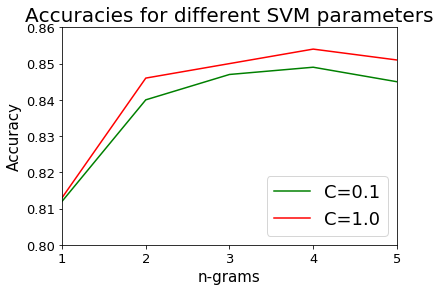
\includegraphics[scale=0.53]{SVM_accuracies}

As we can observe from the figure above, best results were obtained using a \textit{4-gram} representation and with a higher value of the parameter C which represents the regularization parameter for correct classification of training examples. The best results we obtained was with $C=1.0$, although the difference between the different values of \textit{C} proved to be negligible in most iterations.

After SVM, we focused on creating a convolutional neural network (CNN). After some initial testing with different layer configurations, we created a simple architecture with one hidden layer, 128 convolutional filters of sizes {2,3,4,5,6} which is in total 640 filters where each filter is followed by a ReLU activation layer and a max pooling layer. Thanks to the Google Cloud Platform and Nvidia Tesla K80 GPU with 12 GB of GDDR5 memory, we were able to evaluate the effectiveness of our algorithms in a reasonable time and for our best model, run it for 30 epochs, which is approximately 73000 steps. Figure 2 illustrates the training process and shows the train (orange) and validation (blue) scores over time. We evaluated test data on Kaggle after 25000 steps and got a score of 0.86880. In an effort to further test our model since we used our seemingly optimal preprocessing methods at the time, we got our best score after 74000 steps, which is 0.87320. 

\bigskip
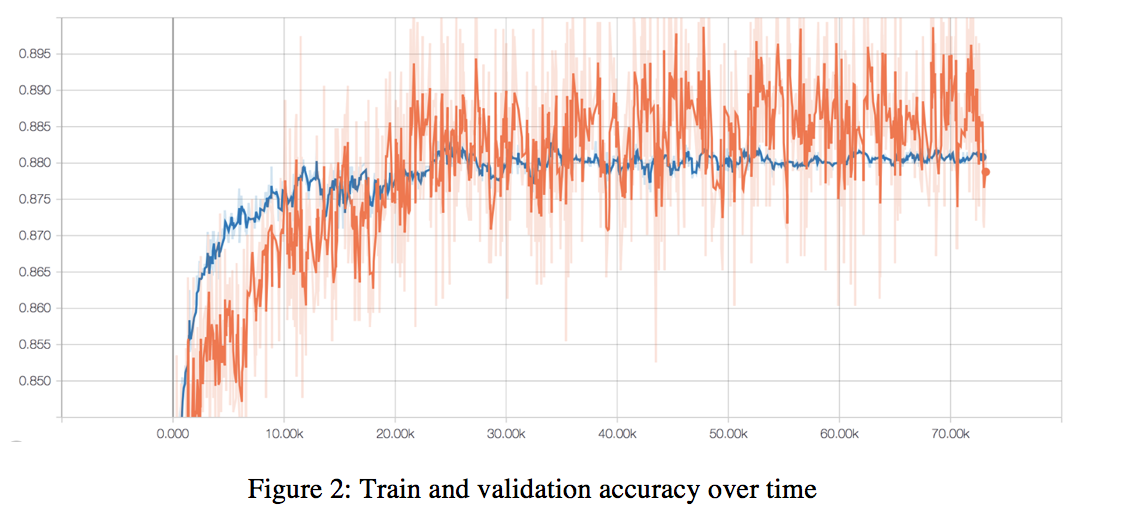
\includegraphics[scale=0.42]{CNN_training}

Additionally, we present below a table showing the accuracies we achieved using and aggregating different preprocessing methods  with our optimal CNN configuration.

\bigskip
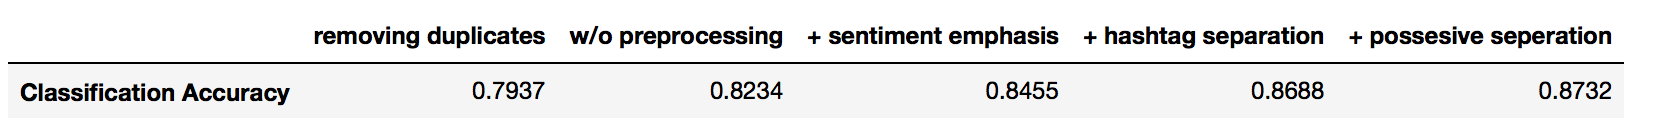
\includegraphics[scale=0.30]{classification_accuracies}
\medskip

\section*{Conclusion}
In conclusion, we realized that sentiment analysis is an arduous task, but one that can provide essential insight into natural language processing and understand how human sentiment is expressed, especially on highly informal media platforms such as Twitter. We learned that preprocessing for such datasets is an essential aspect of proper classification and that different text representations can play crucial roles when combined with powerful algorithms such as SVM and CNN. Ultimately, the highest accuracy score we achieved and were able to reproduce on Kaggle was 0.87320, among the highest for the competition. 

\bibliographystyle{IEEEtran}
\bibliography{literature}

\end{document}